\begin{frame}{Un peu d'histoire}
    \begin{itemize}
        \item mars 2013 : Release par Solomon Hykes (dotcloud)
        \item octobre 2013 : dotcloud devient Docker, Inc
        \item 2014 : passage de Linux containers à libcontainers (Golang)
        \item 2014 : partenariat avec Amazon EC2 et IBM
        \item 2015 : Succès Github (plus de 1100 contributeurs)
        \item 2016 : Windocks, portage du projet à Windows 
        \item 2017 : 13 milliards de téléchargements, + 160\% de mentions sur LinkedIn par rapport à 2016
        \item 2019 : 1917 contributeurs, 43 573 commits
    \end{itemize}
\end{frame}

\begin{frame}{En bref}
\begin{itemize}
    \item Projet Open Source
    \item Gestionnaire de containers
    \item Peut tourner dans une machine virtuelle
    \item Permet de faire tourner des micro services sur une architecture distribuée
\end{itemize}
    
\end{frame}

\begin{frame}{Container}

\begin{block}{}
     Un container est un package exécutable, léger et autonome qui contient tout ce qu'il faut pour faire tourner un logiciel et qui est indépendant du système d'exploitation.
\end{block}

\end{frame}

\begin{frame}{Containers vs Machine Virtuelle}
    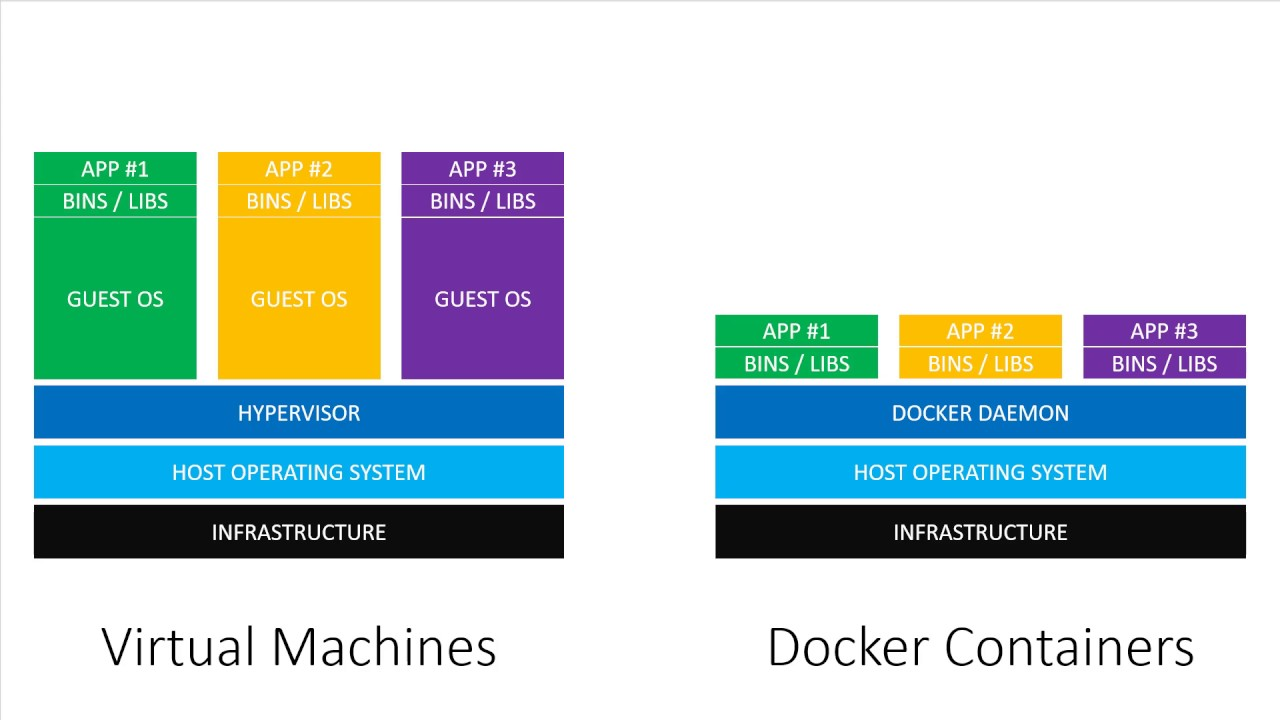
\includegraphics[width=10cm]{img/dockerVSVM.jpg}
\end{frame}